
\documentclass{standalone}
\usepackage{tikz}
\usetikzlibrary{arrows,positioning} 
\tikzset{
    %Define standard arrow tip
    >=stealth',
    %Define style for boxes
    punkt/.style={
           rectangle,
           rounded corners,
           draw=black, thick,
           text width=4.5em,
           minimum height=2em,
           text centered},
    node/.style={
           rectangle,
           rounded corners,
           draw=black, thin,
           text width=3.5em,
           minimum height=2em,
           text centered},
    node/.style={
           rectangle,
           rounded corners,
           draw=black, 
           text width=4.5em,
           minimum height=2em,
           text centered,
           fill={rgb:black,1;white,3}},
    % Define arrow style
    pil/.style={
           ->,
           thick,
           shorten <=2pt,
           shorten >=2pt,}
every node/.style={align=center}           
}

\begin{document}

\begin{tikzpicture}
\node[scale=0.25] at (0,0) {
\begin{tikzpicture}[node distance=1cm, auto,]


%owner
\node[punkt] at (-2,0) (owner) {owner};

%guardian, arrow from owner
\node[punkt, right=2cm of owner] (guardian) {guardian}
  edge[pil, <-] node[auto] {\begin{tabular}{c}\small{store} \\\small{request}\end{tabular}} (owner);

%node after guardian - arrow to node
\node[right=2cm of guardian] (rog) {};
\node[node, below=of rog] (node1) {node}
  edge[pil, <-, bend right=30] node[right=3pt] {forwarding} (guardian.east);

%
\node[node] (node2) at (4,-3) {node}
  (node2.east) edge[pil, <-, dashed, bend right=45] node[right=1pt] {forwarding} (node1.-60);
\node[node] (node3) at (9,-4) {node};
\node[punkt] (retriever) at (10,-1) {retriever}
  edge[pil, ->, bend right=10] node[left=1pt]{retrieval} node[right=1pt]{ request} (node3);
% \node[punkt] (pseudo) at (3.4,-8.8) {closest node};
\node[punkt] (custodian) at (2.5,-6) {custodian}
%   (node4.west) edge[pil,dashed] (custodian)
  (custodian.west) edge[pil, <-, bend left=70] node[auto]{forwarding} (node2.west)
%   (custodian.-15) edge[pil,dashed, bend left=30, <->] node[auto]{
%   \begin{tabular}{c}missing\\ link\end{tabular}
%   }(pseudo)
;
\node[node] (node4) at (8,-6) {node}
  (node4.south west) edge[pil, ->, bend left=45] node[above=1pt]{retrieval}(custodian.south east)
  (node4.north) edge[pil,<-,dashed, bend left=15] node[auto]{forwarding}(node3);

\node (chunklabel) at (3.5,-4) {chunk address};  
\node (chunk) at (4.2,-5.5) {$\bullet$}
 edge[pil, <-] (chunklabel.south);  
% \node[draw, shape=circle, dotted, minimum size=6.5cm] at (chunk) {};

% \node at (5.5,-4.5) {most proximate};




%  %nodes
%  \node[punkt] (market) {Market (b)};
%  \node[punkt, inner sep=5pt,below=0.5cm of market]
%  (formidler) {Intermediaries (c)};
%  % We make a dummy figure to make everything look nice.
%  \node[above=of market] (dummy) {};
%  \node[right=of dummy] (t) {Ultimate borrower}
%    edge[pil,bend left=45] (market.east) % edges are used to connect two nodes
%    edge[pil, bend left=45] (formidler.east); % .east since we want
%                                              % consistent style
%  \node[left=of dummy] (g) {Ultimate lender}
%    edge[pil, bend right=45] (market.west)
%    edge[pil, bend right=45] (formidler.west)
%    edge[pil,<->, bend left=45] node[auto] {Direct (a)} (t);
\end{tikzpicture}

};
% \node[scale=0.25] at (3,0) {
% 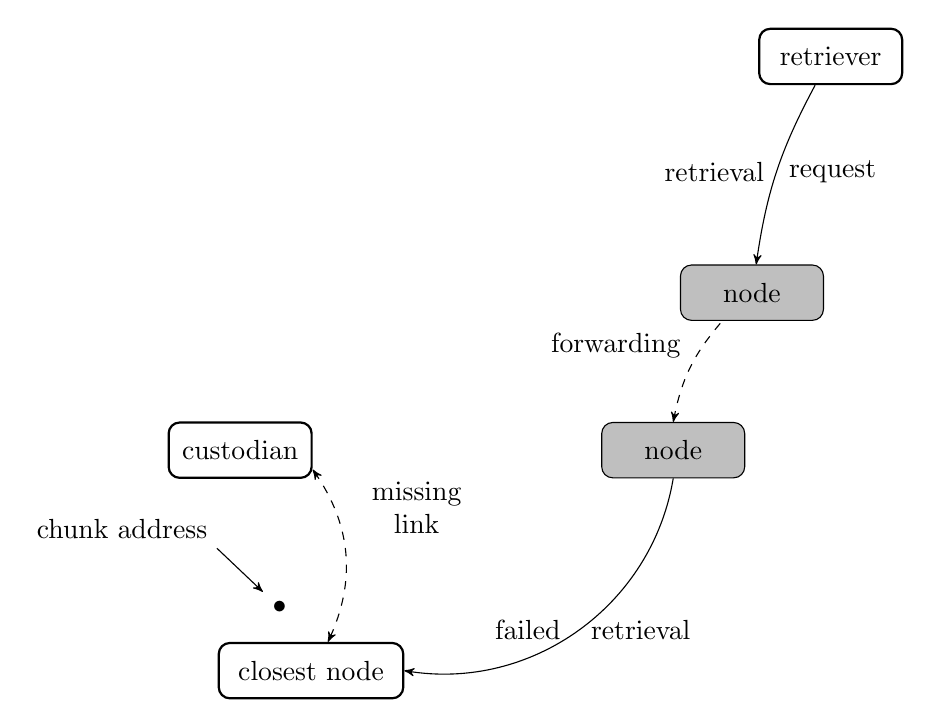
\begin{tikzpicture}[node distance=1cm, auto,]


%owner
% \node[punkt] at (-2,0) (owner) {owner};
% \node at (-2,0) (owner){};
%guardian, arrow from owner
% \node[punkt, right=2cm of owner] (guardian) {guardian}
%   edge[pil, <-] node[auto] {\begin{tabular}{c}\small{store} \\\small{request}\end{tabular}} (owner)
;

%node after guardian - arrow to node
% \node[right=2cm of guardian] (rog) {};
% \node[node, below=of rog] (node1) {node}
%   (node1.west) edge[pil, <-, bend left=45] node[left=3pt] {finger point} (guardian.south)
;

  
\node[punkt, text width=6em] (pseudo) at (3.4,-8.8) {closest node};  
%
% \node[node] (node2) at (4,-3) {node}
%   (node2.east) edge[pil, <-, dashed, bend right=45] node[right=1pt] {finger point} (node1.-60);
\node[node] (node3) at (9,-4) {node};
\node[punkt] (retriever) at (10,-1) {retriever}
  edge[pil, ->, bend right=10] node[left=1pt]{retrieval} node[right=1pt]{ request} (node3);
% \node[punkt] (pseudo) at (3.4,-8.8) {closest node};
\node[punkt] (custodian) at (2.5,-6) {custodian}
(custodian.-15) edge[pil,dashed, bend left=30, <->] node[auto]{
  \begin{tabular}{c}missing\\ link\end{tabular}
  }(pseudo)
%   (node4.west) edge[pil,dashed] (custodian)
%   (custodian.west) edge[pil, <-, bend left=70] node[auto]{finger point} (node2.west)
%   (custodian.-15) edge[pil,dashed, bend left=30, <->] node[auto]{
%   \begin{tabular}{c}missing\\ link\end{tabular}
%   }(pseudo)
;
\node[node] (node4) at (8,-6) {node}
  (node4.south) edge[pil, ->, bend left=45] node[left=3pt]{failed}node[right=1pt]{ retrieval}(pseudo.east)
  (node4.north) edge[pil,<-,dashed, bend left=15] node[auto]{forwarding}(node3);

% \node (chunklabel) at (3.5,-4) {chunk address};  
% \node (chunk) at (4.2,-5.5) {$\bullet$}
%  edge[pil, <-] (chunklabel.south);  
% \node[draw, shape=circle, dotted, minimum size=6.5cm] at (chunk) {};

% \node at (5.5,-4.5) {most proximate};

\node (chunklabel) at (1,-7) {chunk address};  
\node (chunk) at (3,-8) {$\bullet$}
 edge[pil, <-] (chunklabel.south east)
 
 ;  



\end{tikzpicture}

% };
% \node[scale=0.25] at (6,0) {
% 
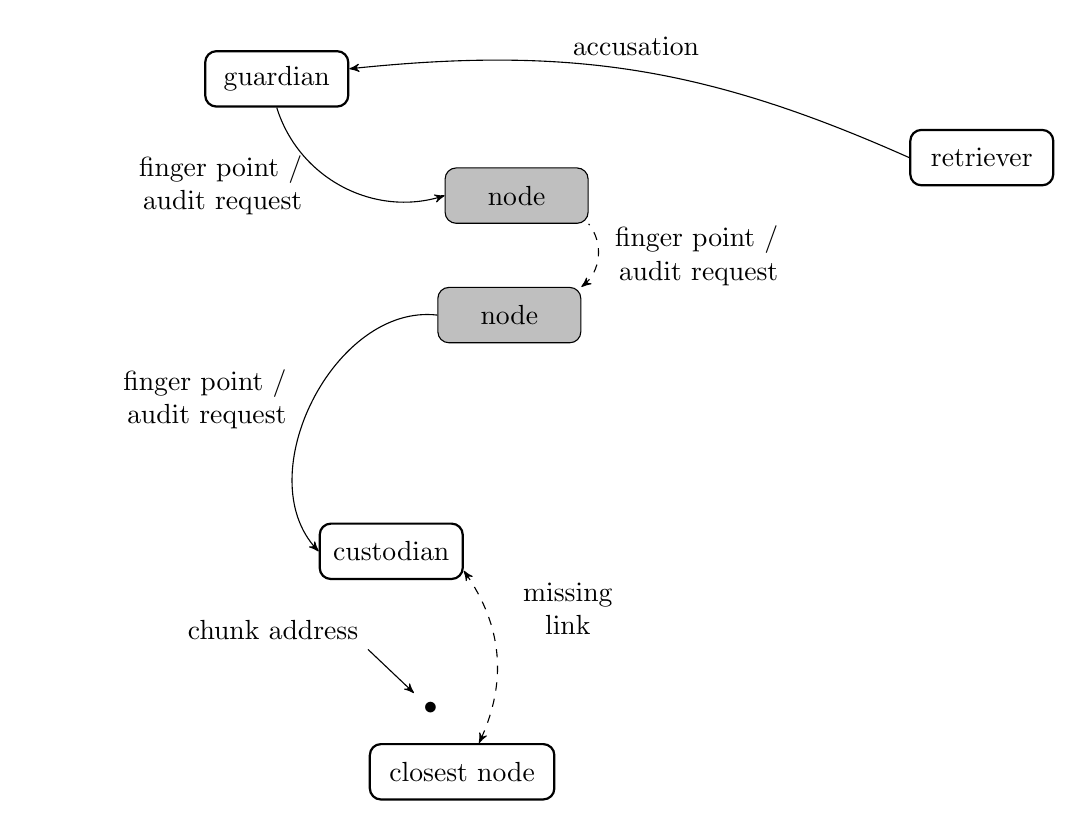
\begin{tikzpicture}[node distance=1cm, auto,]


%owner
% \node[punkt] at (-2,0) (owner) {owner};
\node at (-2,0) (owner){};
%guardian, arrow from owner
\node[punkt, right=2cm of owner] (guardian) {guardian}
%   edge[pil, <-] node[auto] {\begin{tabular}{c}\small{store} \\\small{request}\end{tabular}} (owner)
;

%node after guardian - arrow to node
\node[right=2cm of guardian] (rog) {};
\node[node, below=of rog] (node1) {node}
  (node1.west) edge[pil, <-, bend left=45] node[left=5pt] {\begin{tabular}{r}finger point /\\\quad audit request\end{tabular}} (guardian.south);

  
\node[punkt, text width=6em] (pseudo) at (3.4,-8.8) {closest node};  
%
\node[node] (node2) at (4,-3) {node}
  (node2.north east) edge[pil, <-, dashed, bend right=45] node[right=-12pt] {
  \begin{tabular}{r}finger point /\\\quad audit request\end{tabular}
  } (node1.south east);
% \node[node] (node3) at (9,-4) {node};
\node[punkt] (retriever) at (10,-1) {retriever}
%   edge[pil, ->, bend right=10] node[left=1pt]{retrieval} node[right=1pt]{ request} (node3)
  ;
% \node[punkt] (pseudo) at (3.4,-8.8) {closest node};
\node[punkt] (custodian) at (2.5,-6) {custodian}
(custodian.-15) edge[pil,dashed, bend left=30, <->] node[auto]{
  \begin{tabular}{c}missing\\ link\end{tabular}
  }(pseudo)
%   (node4.west) edge[pil,dashed] (custodian)
  (custodian.west) edge[pil, <-, bend left=70] node[left]{\begin{tabular}{r}finger point /\\\quad audit request\end{tabular}} (node2.west)
%   (custodian.-15) edge[pil,dashed, bend left=30, <->] node[auto]{
%   \begin{tabular}{c}missing\\ link\end{tabular}
%   }(pseudo)
;
% \node[node] (node4) at (8,-6) {node}
%   (node4.south) edge[pil, ->, bend left=45] node[left=3pt]{failed}node[right=1pt]{ retrieval}(pseudo.east)
%   (node4.north) edge[pil,<-,dashed, bend left=15] node[auto]{forwarding}(node3);

% \node (chunklabel) at (3.5,-4) {chunk address};  
% \node (chunk) at (4.2,-5.5) {$\bullet$}
%  edge[pil, <-] (chunklabel.south);  
% \node[draw, shape=circle, dotted, minimum size=6.5cm] at (chunk) {};

% \node at (5.5,-4.5) {most proximate};

\node (chunklabel) at (1,-7) {chunk address};  
\node (chunk) at (3,-8) {$\bullet$}
 edge[pil, <-] (chunklabel.south east)
 (retriever.west) edge[pil, ->, bend right=15] node[above=2pt]{accusation} (guardian)
 
 
 ;  

\end{tikzpicture}

% };
\end{tikzpicture}
\end{document}
